\chapter{Introduction}
Since their first development in the 1960s, \emph{\ooo} (also known as \emph{dynamic scheduling}) microprocessors have become the main architectural paradigm used in high-performance CPUs, given their ability to hide pipeline latencies and allow for a faster program execution. Along with that, another key role in achieving high effective performance is played by the concept of \emph{speculation} and in particular by branch prediction techniques, which improve the pipeline throughput by maintaining a constant instruction flow inside the processor.

Nowadays, almost every device of common use, from desktop computers, to laptops, to smartphones and tablets, contains some kind of \ooo core which exploits such techniques to offer the computing power and pleasant user experience that the modern world demands. Of course, these architectural design choices come with the drawback of significant added hardware complexity, so there are still some very low power or very low cost microprocessors which do not employ them.

In order to deeply understand such complex architectures and explore the design choices that must be faced in order to achieve that final result, a very convenient way is to make use of an open-source \acf{ISA}, namely \riscv, which in turn allows the design of open source hardware. 

This is exactly the aim of this thesis work: to design a \riscv core, featuring \ooo execution and speculation to face the issues that such a project involves firsthand, and gain valuable experience in this field of computer architectures. Given its complexity, this work has been carried out by the candidate along with two other colleagues, each one developing a defined part of the core, to come up with the complete design. It is common hope for this project to also serve as the starting point for the future development of a \riscv based platform at Politecnico di Torino, which could be used for a many different research purposes. For this reason, the entire design and its documentation will be available on a GitHub repository.

\section{The \riscv ISA}
\riscv started as a summer research project in 2010 at UC Berkeley by PhD candidates Andrew Waterman and Yunsup Lee and professors Krste Asanović and David Patterson, but soon developed into a fully featured \ac{ISA}, presented several years later in Waterman's dissertation \cite{waterman}. \todo{Why a new ISA from scratch?}

Today the goal of \riscv is to become a universal \ac{ISA} \cite{reader}, able to suit all kinds of processors, from small embedded ones to high-performance cores, from single issue in-order to superscalar out-of-order microarchitectures. Moreover, it is also designed to be implementation independent, in order to work on FPGA, ASIC and even future technologies, and to be compatible with a large number of popular softwares and programming languages.

How \riscv intends to achieve that is by leveraging its two main strengths: first of all it is a completely \emph{open source} \ac{ISA}, meaning that no single company has control over its development and future, and secondly it is \emph{modular}, in the sense that the base instructions are frozen and will stay the same, while new extensions are available and will be developed to expand the capabilities of the ISA (see section \ref{sec:extensions}).

\riscv belongs to a non-profit foundation, composed by many different corporate members as well as other non-profits and academic institutions, which together aim at maintaining the stability of the \ac{ISA}, evolving it when necessary and trying to make it ever more popular. For more information, refer to \url{https://riscv.org/}.\todo[inline]{Add other advantages of the ISA (see Reader chapter 1)}

\subsection{Extensions}\label{sec:extensions}
Most \acp{ISA} are \emph{incremental}, meaning that, in order to ensure compatibility, every new processor must implement new \ac{ISA} extensions as well as all the extensions introduced in the past, which leads to an accumulation of very rarely used instructions and a subsequent waste of hardware complexity and area. A clear example of this inflation is the growth of the number of instructions in the x86 \ac{ISA} (figure \ref{fig:x86}).
  
\begin{figure}[hbtp]
  \centering
  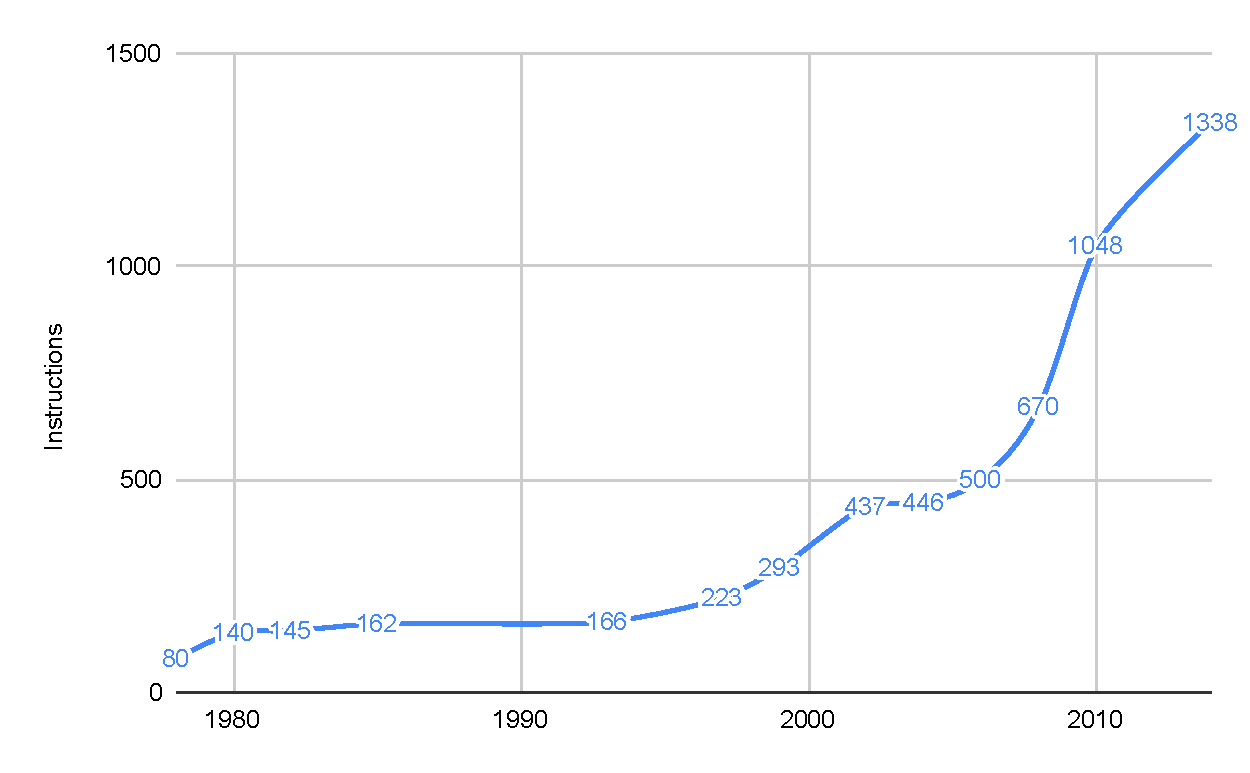
\includegraphics[width=0.8\textwidth]{img/x86.pdf}
  \caption[x86 instruction count over time]{x86 instruction count over time\footnotemark}
  \label{fig:x86}
\end{figure}
\footnotetext{Data taken from \cite[p.~3]{reader}}

One the other hand, as stated above, \riscv is a \emph{modular} \ac{ISA}: a small number of base instructions (called RV32I, RV64I or RV128I for 32, 64 and 128-bit processors respectively) must be implemented by all instances of \riscv processors and are guaranteed to never change in the future, while on top of that, designers can freely choose to include support or not for each of the other optional extensions, some of which have already been frozen, while others are still in development. Table \ref{tab:extensions} contains a list of available extensions at the time of writing.

\begin{table}[hbtp]
  \centering
  \rowcolors{1}{}{gray!10}
  \begin{tabular}{p{\dimexpr 0.2\linewidth-2\tabcolsep}
                  p{\dimexpr 0.8\linewidth-2\tabcolsep}}
    \toprule
    \textbf{Name} & \textbf{Description} \\
    \hline
    I             & Base integer instruction set, including arithmetic and logic instructions, jump, branch and control transfer instructions and some miscellaneous general management ones. \\
    M             & Integer multiplication and division extension. \\
    A             & Atomic extension for atomic memory operations, for process synchronization. \\
    F             & Single-precision floating point extension. \\
    D             & Double-precision floating point extension. \\
    G             & Shorthand for all the previous ones. \lens supports the RV64G \ac{ISA}. \\
    Q             & Quad-precision floating point extension. \\
    L             & Decimal floating point extension. \\
    C             & Compressed instructions extension. \\
    B             & Bit manipulation extension. \\
    J             & Dynamically translated languages extension. \\
    T             & Transactional memory extension. \\
    P             & Packed-SIMD extension. \\
    V             & Vector extension. \\
    N             & User-level interrupts extension. \\
    H             & Hypervisor extension. \\
    \bottomrule
  \end{tabular}
  \caption{\riscv \ac{ISA} extensions \cite{reader}}
  \label{tab:extensions}
\end{table}

\subsection{Comparison with other \acsp{ISA}}\label{sec:isas}
Arguably the two most popular \acp{ISA} at the present time are Intel x86 and ARM, which are dominant in the desktop/laptop computers and smartphones/tablets markets respectively. The first significant difference between them and \riscv is that they are \emph{proprietary} \acp{ISA}, which means that whoever wants to design a processor based on such instruction sets is obliged to the payment of the required royalties. On the other hand, \riscv is free for everyone.

For what concerns the microarchitectural standpoint, another major difference resides in the organization of the internal registers. First of all, \riscv has 32 of them, twice as much as ARM has, and four times as much as x86. A higher number of registers greatly simplifies assembly language programming and compiler writing. Moreover, the first of those registers, register \texttt{x0}, is hardwired to zero, which allows for a significant reduction in instruction count, as many instructions present in other \acp{ISA}, which do not have a zero register, can be synthesized using RV instructions with \texttt{x0} as an operand. As an example, \riscv does not need a separate instruction in order to branch if the value of a register is zero: this operation can be obtained with the \texttt{beq} (branch if equal) instruction using \texttt{x0} as the second operand. The \ac{PC} in the \riscv \ac{ISA} is a separate register, and that prevents any instruction from being able to modify it and thus become a branch instruction, as is the case of the ARM \ac{ISA}, reducing the complexity of the branch prediction hardware and avoiding the loss of one general purpose register.

By keeping simplicity in mind, \riscv does not provide direct support for byte or half-word integer computation, which can be carried out using separate shift instructions, as they are not critical in terms of efficiency and energy consumption, as are for instance reduced-size memory accesses \cite[p.~20]{reader}. In addition, multiplication and division are not present in the base \ac{ISA} (they are comprised in the M extension), and that means that a full software stack can run even without them, which helps reduce the size of embedded chips where such operations are not needed.

Other instructions that the designers of \riscv chose not to include are, among others, stack instructions, as the stack pointer is one of the general purpose registers and so is accessed as any other register, delayed load, as it is deemed as useless in modern deeply pipelined processors, and finally delayed branch and condition code instructions, which complicate the dependencies checking in \ooo processors \cite[p.~21]{reader}.

It is quite clear that who conceived the \riscv \ac{ISA} adopted a philosophy of keeping it simple and that \emph{less is more}, by targeted choices made by learning from the work achieved in the previous decades.